\documentclass[journal,12pt,twocolumn]{IEEEtran}

\usepackage{graphicx}
\usepackage{setspace}
\usepackage{gensymb}
\singlespacing
\usepackage[cmex10]{amsmath}
\usepackage{amssymb}
\usepackage{xurl}
\usepackage{tabularx}
\usepackage{amsthm}
\usepackage{comment}
\usepackage{mathrsfs}
\usepackage{txfonts}
\usepackage{stfloats}
\usepackage{bm}
\usepackage{cite}
\usepackage{cases}
\usepackage{subfig}
\usepackage{arydshln}
\usepackage{longtable}
\usepackage{multirow}

\usepackage{enumitem}
\usepackage{mathtools}
\usepackage{steinmetz}
\usepackage{tikz}
\usepackage{circuitikz}
\usepackage{verbatim}
\usepackage{tfrupee}
\usepackage[breaklinks=true]{hyperref}
\usepackage{graphicx}
\usepackage{tkz-euclide}
\usetikzlibrary{automata, positioning}
\usetikzlibrary{calc,math}
\usepackage{listings}
    \usepackage{color}                                            %%
    \usepackage{array}                                            %%
    \usepackage{longtable}                                        %%
    \usepackage{calc}                                             %%
    \usepackage{multirow}                                         %%
    \usepackage{hhline}                                           %%
    \usepackage{ifthen}                                           %%
    \usepackage{lscape}     
\usepackage{multicol}
\usepackage{chngcntr}
\usepackage{blkarray}

\DeclareMathOperator*{\Res}{Res}

\renewcommand\thesection{\arabic{section}}
\renewcommand\thesubsection{\thesection.\arabic{subsection}}
\renewcommand\thesubsubsection{\thesubsection.\arabic{subsubsection}}

\renewcommand\thesectiondis{\arabic{section}}
\renewcommand\thesubsectiondis{\thesectiondis.\arabic{subsection}}
\renewcommand\thesubsubsectiondis{\thesubsectiondis.\arabic{subsubsection}}


\hyphenation{op-tical net-works semi-conduc-tor}
\def\inputGnumericTable{}                                 %%

\lstset{
%language=C,
frame=single, 
breaklines=true,
columns=fullflexible
}
\begin{document}


\newtheorem{theorem}{Theorem}[section]
\newtheorem{problem}{Problem}
\newtheorem{proposition}{Proposition}[section]
\newtheorem{lemma}{Lemma}[section]
\newtheorem{corollary}[theorem]{Corollary}
\newtheorem{example}{Example}[section]
\newtheorem{definition}[problem]{Definition}

\newcommand{\BEQA}{\begin{eqnarray}}
\newcommand{\EEQA}{\end{eqnarray}}
\newcommand{\define}{\stackrel{\triangle}{=}}
\bibliographystyle{IEEEtran}
\raggedbottom
\setlength{\parindent}{0pt}
\providecommand{\mbf}{\mathbf}
\providecommand{\pr}[1]{\ensuremath{\Pr\left(#1\right)}}
\providecommand{\qfunc}[1]{\ensuremath{Q\left(#1\right)}}
\providecommand{\sbrak}[1]{\ensuremath{{}\left[#1\right]}}
\providecommand{\lsbrak}[1]{\ensuremath{{}\left[#1\right.}}
\providecommand{\rsbrak}[1]{\ensuremath{{}\left.#1\right]}}
\providecommand{\brak}[1]{\ensuremath{\left(#1\right)}}
\providecommand{\lbrak}[1]{\ensuremath{\left(#1\right.}}
\providecommand{\rbrak}[1]{\ensuremath{\left.#1\right)}}
\providecommand{\cbrak}[1]{\ensuremath{\left\{#1\right\}}}
\providecommand{\lcbrak}[1]{\ensuremath{\left\{#1\right.}}
\providecommand{\rcbrak}[1]{\ensuremath{\left.#1\right\}}}
\theoremstyle{remark}
\newtheorem{rem}{Remark}
\newcommand{\sgn}{\mathop{\mathrm{sgn}}}
\providecommand{\abs}[1]{\vert#1\vert}
\providecommand{\res}[1]{\Res\displaylimits_{#1}} 
\providecommand{\norm}[1]{\lVert#1\rVert}
%\providecommand{\norm}[1]{\lVert#1\rVert}
\providecommand{\mtx}[1]{\mathbf{#1}}
\providecommand{\mean}[1]{E[ #1 ]}
\providecommand{\fourier}{\overset{\mathcal{F}}{ \rightleftharpoons}}
%\providecommand{\hilbert}{\overset{\mathcal{H}}{ \rightleftharpoons}}
\providecommand{\system}{\overset{\mathcal{H}}{ \longleftrightarrow}}
	%\newcommand{\solution}[2]{\textbf{Solution:}{#1}}
\newcommand{\solution}{\noindent \textbf{Solution: }}
\newcommand{\cosec}{\,\text{cosec}\,}
\providecommand{\dec}[2]{\ensuremath{\overset{#1}{\underset{#2}{\gtrless}}}}
\newcommand{\myvec}[1]{\ensuremath{\begin{pmatrix}#1\end{pmatrix}}}
\newcommand{\mydet}[1]{\ensuremath{\begin{vmatrix}#1\end{vmatrix}}}
\newcommand*{\permcomb}[4][0mu]{{{}^{#3}\mkern#1#2_{#4}}}
\newcommand*{\perm}[1][-3mu]{\permcomb[#1]{P}}
\newcommand*{\comb}[1][-1mu]{\permcomb[#1]{C}}
\numberwithin{equation}{subsection}
\makeatletter
\@addtoreset{figure}{problem}
\makeatother
\let\StandardTheFigure\thefigure
\let\vec\mathbf
\renewcommand{\thefigure}{\theproblem}
\def\putbox#1#2#3{\makebox[0in][l]{\makebox[#1][l]{}\raisebox{\baselineskip}[0in][0in]{\raisebox{#2}[0in][0in]{#3}}}}
     \def\rightbox#1{\makebox[0in][r]{#1}}
     \def\centbox#1{\makebox[0in]{#1}}
     \def\topbox#1{\raisebox{-\baselineskip}[0in][0in]{#1}}
     \def\midbox#1{\raisebox{-0.5\baselineskip}[0in][0in]{#1}}
\vspace{3cm}
\title{\textbf{ GATE ASSIGNMENT 4}}
\author{Dhatri Nanda - AI20BTECH11002}
\maketitle
\newpage
\bigskip
\renewcommand{\thefigure}{\arabic{figure}}
\renewcommand{\thetable}{\arabic{table}}
Download latex-tikz codes from 
%
\begin{lstlisting}
https://github.com/Dhatri-nanda/EE3900/blob/main/Gate_4/Gate_4.tex
\end{lstlisting}
\section*{QUESTION}
The Fourier Transform of the signal $f(t) = e^{-3t^2}$ is of the following form, where A and B are constants

\begin{enumerate}[label={\Alph*)}]
\item $Ae^{-B|f|}$\\
\item $Ae^{-Bf^2}$\\
\item $A + B|f|^2$\\
\item $Ae^{-Bf}$\\
\end{enumerate}
\section*{SOLUTION}
 The fourier transform of a given signal f(t) is given by,
        \begin{align}
            X(f) = \int_{-\infty}^{\infty} f(t) e^{-2\pi jft} dt
        \end{align}
\begin{lemma}
If a signal $f(t)$ has a fourier transform $F(f)$, then
\begin{align}
    f'(t) \fourier 2\pi jfF(f) 
\end{align}\label{lemma 1}
\end{lemma}
\begin{proof}
 The fourier transform of $\frac{d f(t)}{dt}$ is given by,
        \begin{align}
            &= \int_{-\infty}^{\infty}  \frac{df(t)}{dt} e^{-2\pi jft} dt\\
            &= \sbrak{e^{-2\pi jft} f(t)}_{-\infty}^{\infty} + 2\pi jf\int_{-\infty}^{\infty} f(t) e^{-2\pi jft} dt\\
            &= 2\pi jfF(f)
        \end{align}
\end{proof}
\begin{lemma}
If a signal f(t) has fourier transform F(f) then,
\begin{align}
    tf(t) \fourier \frac{j}{2\pi}F^{'}(f) 
\end{align} \label{lemma 2}
\end{lemma}
\begin{proof}
 We prove it by finding the inverse fourier transform of $\frac{j}{2\pi}\frac{dF(f)}{df}$
        
        The inverse fourier transform is given by
        \begin{align}
            f_1(t) &= \int_{-\infty}^{\infty} F_1(f)e^{j2\pi ft} df\\\label{eq 0.0.7}
            &= \frac{1}{2\pi} \int_{-\infty}^{\infty} j\frac{dF(f)}{df}
            e^{j2\pi ft} df\\
            &= \frac{1}{2\pi} \sbrak{je^{j2\pi ft} F(f)}_{-\infty}^{\infty} + \frac{1}{2\pi} \int_{-\infty}^{\infty} te^{j2\pi ft} F(f) df \\
            &= \frac{1}{2\pi} \int_{-\infty}^{\infty} t F(f) e^{j2\pi ft} df 
        \end{align}
        From \eqref{eq 0.0.7}, 
        \begin{align}
            f_1(t) &= tf(t)
        \end{align}
\end{proof}

If we consider the signal
\begin{align}
    f(t) = e^{-\pi t^2}
\end{align}
On differentiating,
\begin{align}
     f'(t) &= e^{-\pi t^2}\times(-2\pi t)\\
    \implies f'(t) &= f(t)\times (-2\pi t)
\end{align}
By applying fourier transformations using lemmas \ref{lemma 1} and \ref{lemma 2}
\begin{align}
    2\pi jfF(f) &= \frac{j}{2\pi}F^{'}(f) \times (-2\pi)\\
    \implies \frac{F'(f)}{F(f)} &= -2\pi f
\end{align}
On integrating,
\begin{align}
    log(F(f)) = \frac{-2\pi f^2}{2}
\end{align}
So, the fourier transform of the signal $f(t) = e^{-\pi t^2}$is
\begin{align}
    F(f) = e^{-\pi f^2}
\end{align}
We know that, if 
\begin{align}
    f(t) &\fourier F(f)\\
    \implies f(at) &\fourier \frac{1}{a}F(f/a)
\end{align}

On substituting $a = \sqrt{3/\pi}$, the fourier transform of the signal $f(t) = e^{-3t^2}$ is 
\begin{align}
   F(f) =  \frac{\sqrt{\pi}}{\sqrt{3}}e^{-\pi^2 f^2/3}
\end{align}

It is of the form 
\begin{align}
    Ae^{-Bf^2} 
\end{align}
where
\begin{align}
    A &= \frac{\sqrt{\pi}}{\sqrt{3}}\\
    B &= \frac{\pi^2}{3}
\end{align}
So, correct option is B

\begin{figure}[htp]
    \centering
    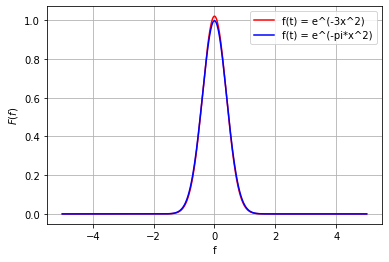
\includegraphics[width=\columnwidth]{fourier.png}
    \caption{plot of fourier transforms}
    \label{fig:my_label}
\end{figure}
\end{document}
